\section*{Nabíjeni}
\addcontentsline{toc}{section}{Nabíjeni}

Aby se dveře trezoru nemuseli pokaždé rozebírat kvůli nabíjení, je deska vybavena lineární nabíječkou 
\href{https://datasheet.lcsc.com/szlcsc/Seaward-Elec-SE9017-HF_C115752.pdf}{SE9017}. 
Tuto nabíjecí obvod jsem zvolil z~nabídky JLCPCB kvůli volitelnému nabíjecímu proudu, který jsem pomocí R48 stanovil na 700 mA, a~také, kvůli malému 
pouzdru a~nízké ceně.
Pro signalizaci zda je~baterie dobita nebo zda se ještě dobijí jsou zde dvě LED~diodi LED4 a~LED5. Když se baterie dobíjí tak svítí LED4, která svítí 
červená, a~když je~baterie dobita svítí LED5, která svítí modře.

\begin{figure}[htbp]
    \centering
    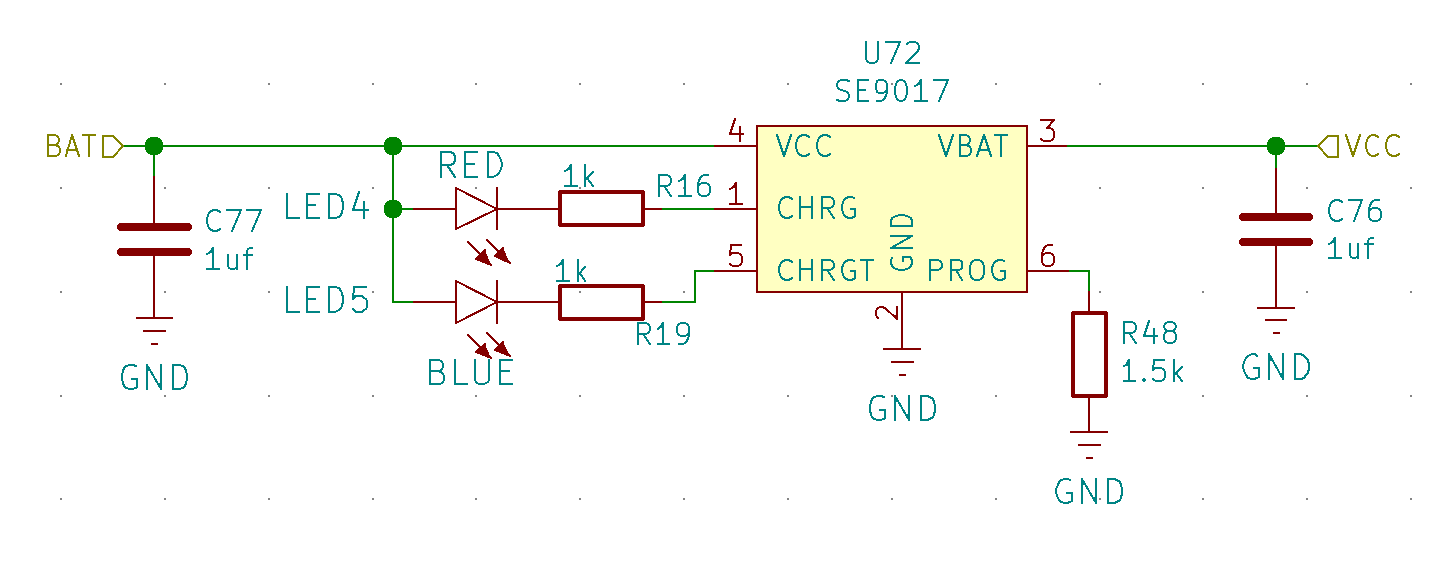
\includegraphics[width=\textwidth]{kapitoly/obrazky/E4/nabijeni/nabijecka.png}
    \caption{zapojeni nabíječky}
    \label{fig:E4-step-up}
\end{figure}

\newpage
% nenapadá mě co víc říct?